\documentclass[border=4pt,varwidth=6in]{standalone}
\usepackage[T1]{fontenc}
\usepackage{mathptmx}
\usepackage[scaled=0.92]{helvet}
\usepackage{courier}
\usepackage{setspace}
\usepackage{amsmath,amssymb,amsthm}
\usepackage{xcolor}
\usepackage{graphicx}
\usepackage{float}
\usepackage[font={singlespacing,normalsize},labelfont=bf,labelsep=period,justification=justified,singlelinecheck=false]{caption}
\usepackage{subcaption}
\usepackage{booktabs,multirow,longtable,threeparttable,array,tabularx}
\usepackage{enumitem}
%% preamble.tex — packages and macros shared by all chapters
% Engine compatibility: biber writes UTF-8 into the .bbl. Under pdfTeX, inputenc maps
% characters outside Latin-1 to T1 glyphs; under XeTeX (tectonic) they would be silently
% dropped from the 8-bit Times fonts, so map them explicitly.
\usepackage{iftex}
\ifXeTeX
  \usepackage{newunicodechar}
  \newunicodechar{č}{\v{c}}\newunicodechar{Č}{\v{C}}\newunicodechar{ě}{\v{e}}\newunicodechar{ř}{\v{r}}
  \newunicodechar{š}{\v{s}}\newunicodechar{Š}{\v{S}}\newunicodechar{ž}{\v{z}}\newunicodechar{Ž}{\v{Z}}
  \newunicodechar{Ł}{\L{}}\newunicodechar{ł}{\l{}}\newunicodechar{ń}{\'n}\newunicodechar{ś}{\'s}
  \newunicodechar{ć}{\'c}\newunicodechar{ż}{\.z}\newunicodechar{ź}{\'z}\newunicodechar{ę}{\k{e}}\newunicodechar{ą}{\k{a}}
  \newunicodechar{ő}{\H{o}}\newunicodechar{ű}{\H{u}}\newunicodechar{ğ}{\u{g}}\newunicodechar{ş}{\c{s}}\newunicodechar{ı}{\i}
\fi
\usepackage{physics}          % \ket, \bra, \expval, \dd, \abs, \norm
\usepackage{bm}
\usepackage{mathtools}
\usepackage{siunitx}
\sisetup{detect-all,per-mode=symbol,range-phrase=--,range-units=single}
\usepackage{tikz}
\usetikzlibrary{quantikz2}
\usetikzlibrary{arrows.meta,positioning,calc,shapes.geometric,fit,backgrounds,matrix,decorations.pathreplacing}
\usepackage{pgfplots}
\pgfplotsset{compat=1.18}
\usepgfplotslibrary{groupplots,fillbetween}
\usepackage[ruled,vlined,linesnumbered]{algorithm2e}
\SetAlFnt{\singlespacing\small}
% cleveref is loaded by ttuthesis.cls *before* algorithm2e, so its algorithm2e alias is never
% installed; name the algocf label type explicitly so \cref{alg:...} prints "Algorithm N".
\usepackage{listings}
\lstset{basicstyle=\ttfamily\footnotesize\singlespacing,breaklines=true,columns=fullflexible,
        keepspaces=true,frame=single,framerule=0.3pt,xleftmargin=1em,showstringspaces=false,
        commentstyle=\itshape\color{black!60},keywordstyle=\bfseries}
\lstdefinelanguage{qasm}{morekeywords={OPENQASM,include,qubit,bit,h,cx,rz,ry,measure,reset,barrier},sensitive=true,morecomment=[l]{//}}

% Theorem-like environments (numbered per chapter, Arabic chapter number)

% Color-blind-safe palette for plots (also varies markers/line styles: TTU accessibility rule)
\definecolor{cbBlue}{HTML}{0072B2}
\definecolor{cbOrange}{HTML}{E69F00}
\definecolor{cbGreen}{HTML}{009E73}
\definecolor{cbRed}{HTML}{D55E00}
\definecolor{cbPurple}{HTML}{CC79A7}
\definecolor{cbSky}{HTML}{56B4E9}
\definecolor{cbGray}{HTML}{555555}
\pgfplotscreateplotcyclelist{ttu}{%
  {cbBlue,mark=*,solid},{cbOrange,mark=square*,dashed},{cbGreen,mark=triangle*,dotted},
  {cbRed,mark=diamond*,dashdotted},{cbPurple,mark=pentagon*,densely dashed},{cbGray,mark=o,loosely dotted}}
\pgfplotsset{every axis/.append style={cycle list name=ttu,width=0.8\linewidth,height=0.5\linewidth,
  tick label style={font=\small},label style={font=\small},legend style={font=\footnotesize,cells={anchor=west}},
  grid=major,grid style={black!12}}}

% Domain macros
\newcommand{\qgear}{Q-GEAR}
\newcommand{\deal}{DEAL}
\newcommand{\qawa}{QAWA}
\newcommand{\qpie}{QPIE}
\newcommand{\vqt}{VQT}
\newcommand{\shardq}{ShardQ}
\newcommand{\nnqa}{NNQA}
\newcommand{\rubriq}{RubriQ}
\newcommand{\cudaq}{CUDA-Q}
\newcommand{\qiskit}{Qiskit}
\newcommand{\qcrank}{QCrank}
\newcommand{\bigO}[1]{\mathcal{O}\!\left(#1\right)}
\newcommand{\Hcost}{H_C}
\newcommand{\Hmix}{H_M}
\newcommand{\code}[3]{[[#1,#2,#3]]}
\newcommand{\eps}{\varepsilon}
\newcommand{\R}{\mathbb{R}}
\newcommand{\C}{\mathbb{C}}
\newcommand{\Z}{\mathbb{Z}}
% \Tr provided by physics
\DeclareMathOperator{\poly}{poly}
\DeclareMathOperator*{\argmin}{arg\,min}
\DeclareMathOperator*{\argmax}{arg\,max}

\newcommand{\todo}[1]{{\color{red!70!black}\textbf{[TODO: #1]}}}
\providecommand{\cref}[1]{#1}
\providecommand{\Cref}[1]{#1}
\providecommand{\labelcref}[1]{#1}
\providecommand{\ref}[1]{#1}
\providecommand{\cite}[1]{[#1]}
\begin{document}
\begin{figure}[H]
\centering
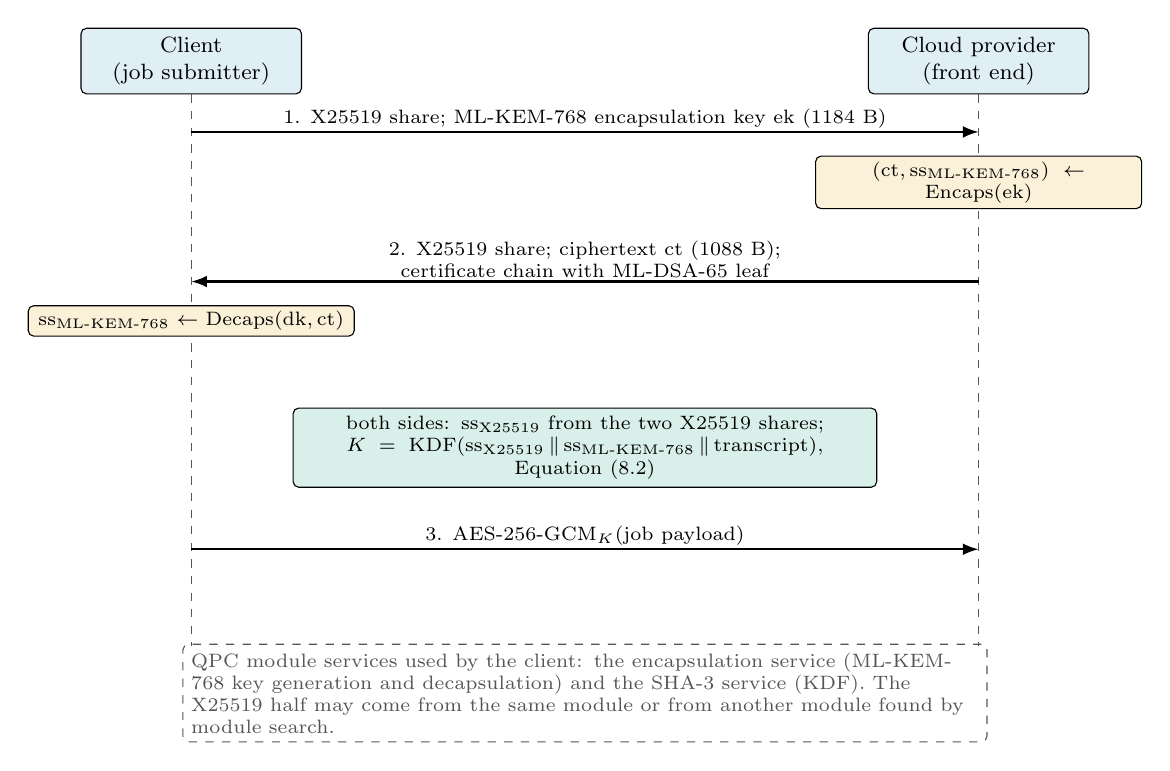
\begin{tikzpicture}[font=\footnotesize,
  life/.style={draw,rounded corners=2pt,fill=cbBlue!12,align=center,minimum width=28mm,minimum height=8mm},
  msg/.style={-{Latex[length=2mm]},thick},
  lbl/.style={font=\scriptsize,align=center,fill=white,inner sep=1pt},
  act/.style={draw,rounded corners=2pt,fill=cbOrange!15,align=center,font=\scriptsize,inner sep=2pt,text width=40mm},
  key/.style={draw,rounded corners=2pt,fill=cbGreen!15,align=center,font=\scriptsize,inner sep=3pt,text width=72mm},
  note/.style={draw,cbGray,dashed,rounded corners=2pt,align=left,font=\scriptsize,inner sep=3pt,text width=100mm}]
  \node[life] (C) at (0,0) {Client\\ (job submitter)};
  \node[life] (P) at (100mm,0) {Cloud provider\\ (front end)};
  \foreach \n in {C,P}{\draw[cbGray,dashed] (\n.south) -- ++(0,-70mm);}
  \draw[msg] (C.south|-0,-9mm) -- (P.south|-0,-9mm) node[lbl,midway,above]{1. X25519 share; ML-KEM-768 encapsulation key $\mathrm{ek}$ (1184 B)};
  \node[act,anchor=north] at (P.south|-0,-12mm) {$(\mathrm{ct},\mathrm{ss}_{\text{ML-KEM-768}}) \leftarrow \mathrm{Encaps}(\mathrm{ek})$};
  \draw[msg] (P.south|-0,-28mm) -- (C.south|-0,-28mm) node[lbl,midway,above]{2. X25519 share; ciphertext $\mathrm{ct}$ (1088 B);\\ certificate chain with ML-DSA-65 leaf};
  \node[act,anchor=north] at (C.south|-0,-31mm) {$\mathrm{ss}_{\text{ML-KEM-768}} \leftarrow \mathrm{Decaps}(\mathrm{dk},\mathrm{ct})$};
  \node[key,anchor=north] at (50mm,-44mm) {both sides: $\mathrm{ss}_{\text{X25519}}$ from the two X25519 shares;\\ $K=\mathrm{KDF}(\mathrm{ss}_{\text{X25519}}\,\|\,\mathrm{ss}_{\text{ML-KEM-768}}\,\|\,\mathrm{transcript})$, Equation (8.2)};
  \draw[msg] (C.south|-0,-62mm) -- (P.south|-0,-62mm) node[lbl,midway,above]{3. AES-256-GCM$_K$(job payload)};
  \node[note,anchor=north] at (50mm,-74mm) {QPC module services used by the client: the encapsulation service (ML-KEM-768 key generation and decapsulation) and the SHA-3 service (KDF). The X25519 half may come from the same module or from another module found by module search.};
\end{tikzpicture}
\end{figure}
\end{document}
